\begin{enumerate}[label=\thesubsection.\arabic*.,ref=\thesubsection.\theenumi]
\numberwithin{equation}{enumi}

\item Sketch the bode magnitude and phase plots for the closed loop (negative feedback) system given by:

\begin{align}
    G\brak{s} = \frac{100\brak{s+2}\brak{s+4}}{s^2 - 3s + 10}
    \label{ee18btech11045_gs}
\end{align}
\begin{align}
    H\brak{s} = \frac{1}{s}
\end{align}

\solution
The system can be represented as:
\begin{figure}[!ht]
	\begin{center}
		\resizebox{\columnwidth}{!}{\tikzstyle{block} = [draw, fill=white, rectangle, 
    minimum height=1cm, minimum width=1cm]
\tikzstyle{sum} = [draw, fill=white, circle, node distance=1cm]
\tikzstyle{input} = [coordinate]
\tikzstyle{output} = [coordinate]
\tikzstyle{pinstyle} = [pin edge={to-,thin,black}]

\begin{tikzpicture}[auto, node distance=2cm,>=latex']

    \node [input, name=input] {X(s)};
    \node [sum, right of=input] (sum) {};
    
    \node [block, right of=sum] (system) {$G(s)$ };
    \node [output, right of=system] (output) {};
    \node [block, below of=system] (measurements) {$H(s)$};

    \draw [draw,->] (input) -- node {$X(s)$} (sum);
    \draw [->] (sum) -- node {} (system);
    \draw [->] (system) -- node [name=y] {$Y(s)$}(output);
    \draw [->] (y) |- (measurements);
    \draw [->] (measurements) -| node[pos=0.99] {$-$} 
        node [near end] {} (sum);
\end{tikzpicture}}
	\end{center}
\caption{Block diagram for the system}
\label{fig:ee18btech11045_1}
\end{figure}

The closed loop transfer function of the system is given by:
\begin{align}
    G_m\brak{s} = \frac{Y\brak{s}}{X\brak{s}} = \frac{G\brak{s}}{1 + G\brak{s}.H\brak{s}}
    \\
    \implies G_m\brak{s} = \frac{100s\brak{s+2}\brak{s+4}}{s^3 + 97s^2 + 610s + 800}
    \label{ee18btech11045_gm}
\end{align}

Evaluate at $s = \j\omega$:
\begin{align}
    G_m\brak{\j\omega} &= \frac{100\j\omega\brak{\j\omega+2}\brak{\j\omega+4}}{\brak{\j\omega}^3 + 97\brak{\j\omega}^2 + 610\brak{\j\omega} + 800}
    \\
    &= \frac{-600\omega^2 + \j\brak{800\omega - 100\omega^3}}{800 - 97\omega^2 + \j\brak{610\omega - \omega^3}}
    \label{ee18btech11045_gmjw}
\end{align}

From \eqref{ee18btech11045_gmjw}:
\begin{align}
    \abs{G_m\brak{\j\omega}} = \frac{\sqrt{\brak{600\omega^2}^2 + \brak{800\omega-100\omega^3}^2}}{\sqrt{\brak{800 - 97\omega^2}^2+\brak{610\omega-\omega^3}^2}}
\end{align}
\begin{multline}
    \phase G_m\brak{\j\omega} = \tan^{-1}\brak{\frac{\omega^2 - 8}{6\omega}}
    \\-\tan^{-1}\brak{\frac{610\omega-\omega^3}{800-97\omega^2}}
\end{multline}    
    

    
The following code plots the bode magnitude and phase plots in Fig. \ref{fig:ee18btech11045_bode1}:

\begin{lstlisting}
codes/ee18btech11045/ee18btech11045_bode1.py
\end{lstlisting}

\begin{figure}[!ht]
\centering
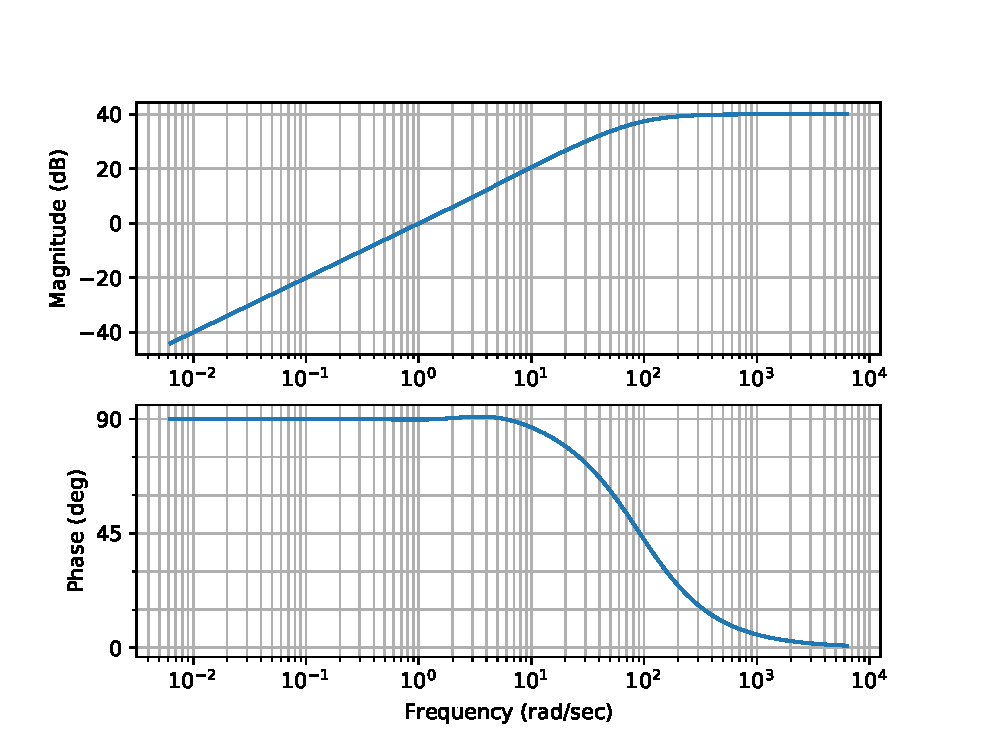
\includegraphics[width=\columnwidth]{./figs/ee18btech11045/ee18btech11045_bode1.eps}
\caption{Bode plot for $G_m(\j\omega)$}
\label{fig:ee18btech11045_bode1}
\end{figure}


\item Compute the gain margin of the system.

\solution

\begin{align}
    G\brak{\j\omega}H\brak{\j\omega} &= \brak{\frac{100\brak{\j\omega+2}\brak{\j\omega+4}}{\brak{\j\omega}^2 - 3\j\omega + 10}}\brak{\frac{1}{\j\omega}}
    \\
    &= \frac{100\brak{-\omega^2 + 8 + \j6\omega}}{3\omega^2+\j\brak{10\omega-\omega^3}}
    \label{ee18btech11045_GHeq}
\end{align}

Using \eqref{ee18btech11045_GHeq}
\begin{align}
    \abs{G\brak{\j\omega}H\brak{\j\omega}} = \frac{100\sqrt{\brak{8-\omega^2}^2 + \brak{6\omega}^2}}{\sqrt{\brak{3\omega^2}^2 + \brak{10\omega - \omega^3}^2}}
    \label{ee18btech11045_gainGH}
\end{align}

\begin{multline}
        \phase G\brak{\j\omega}H\brak{\j\omega} = \tan^{-1}\brak{\frac{6\omega}{8 - \omega^2}} \\ - \tan^{-1}\brak{\frac{10 - \omega^2}{3\omega}}
    \label{ee18btech11045_phaseGH}
\end{multline}

At the phase crossover frequency $\omega_{pc}$:
\begin{align}
    \abs{\phase G\brak{\j\omega}H\brak{\j\omega}} = 180
\end{align}
\begin{align}
    \implies \tan^{-1}\brak{\frac{6\omega_{pc}}{8 - \omega_{pc}^2}} - \tan^{-1}\brak{\frac{10-\omega_{pc}^2}{3\omega_{pc}}} = 180
\end{align}

Solving the above equation:
\begin{align}
    \frac{6\omega_{pc}}{8 - \omega_{pc}^2} = \frac{10-\omega_{pc}^2}{3\omega_{pc}}
\end{align}
\begin{align}
    \implies \omega_{pc} = 5.8 rad/sec
\end{align}
\begin{align}
    \abs{G\brak{\j\omega}H\brak{\j\omega}}_{\omega=\omega_pc} = 28.1 dB
\end{align}

Gain Margin {$GM$} :
\begin{align}
    GM &= 0 - \abs{G\brak{\j\omega}H\brak{\j\omega}}_{\omega=\omega_pc} dB
    \\&= -28.1 dB
\end{align}


\item Compute the phase margin of the system.

\solution

At the gain crossover frequency $\omega_{gc}$:
\begin{align}
    \abs{G\brak{\j\omega}H\brak{\j\omega}}_{\omega=\omega_{gc}} = 1
\end{align}

From \eqref{ee18btech11045_gainGH},
\begin{align}
    10^4\brak{\brak{8-\omega^2}^2 + \brak{6\omega}^2} = 9\omega^4 + \brak{10\omega - \omega^3}^2
\end{align}
\begin{align}
    \implies \omega_{gc} = 100.15 rad/sec
\end{align}

Substitute $\omega_{gc}$ in \eqref{ee18btech11045_phaseGH}:
\begin{align}
    \phase G\brak{\j\omega}H\brak{\j\omega}_{\omega = \omega_{gc}} = 265\degree
\end{align}

Phase Margin {$PM$}:
\begin{align}
    PM &= 180\degree - \phase G\brak{\j\omega}H\brak{\j\omega}_{\omega = \omega_{gc}}
    \\
    &= 180\degree - 265\degree = - 85\degree
\end{align}


\item Verify the values of Gain Margin and Phase Margin using a python plot.

\solution

The following code is used to verify the gain and phase margins:
\begin{lstlisting}
codes/ee18btech11045/ee18btech11045_bode2.py
\end{lstlisting}

\begin{figure}[!ht]
\centering
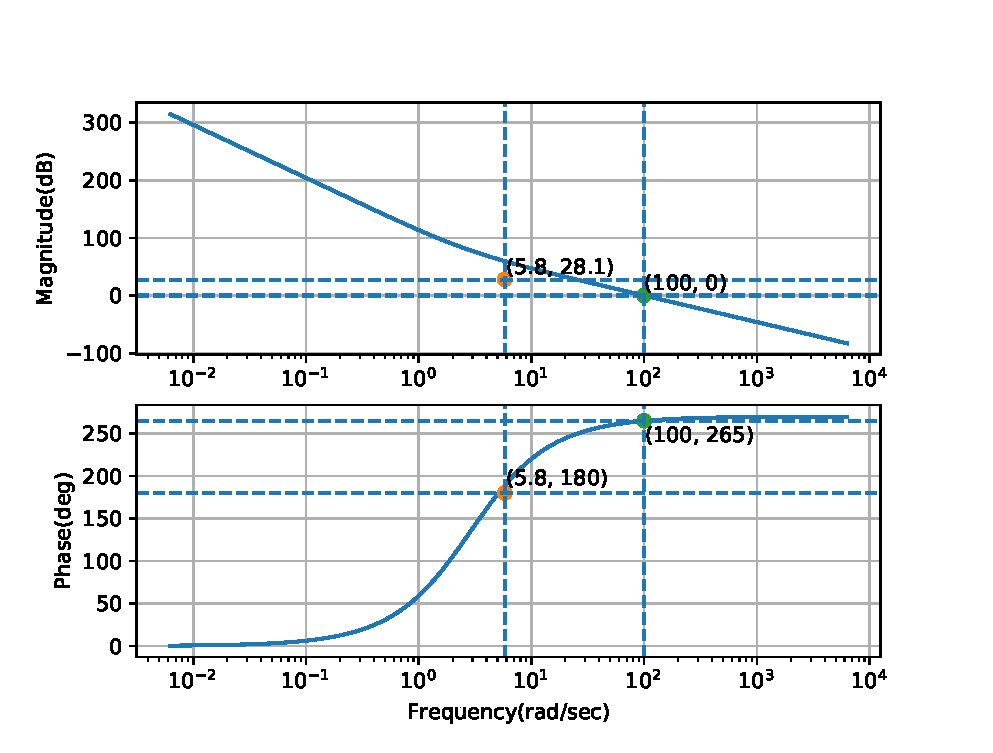
\includegraphics[width=\columnwidth]{./figs/ee18btech11045/ee18btech11045_bode2.eps}
\caption{Bode plot for $G(\j\omega)H(\j\omega)$}
\label{fig:ee18btech11045_bode2}
\end{figure}


\item Comment on the stability of the system

\solution

As both the Gain Margin (GM) and Phase Margin (PM) are found to be negative, the system is unstable.

\end{enumerate}